
\chapter{Tracking and Data Selection}

\section{Reconstruction of SeaQuest Dimuons}

Once the raw hit and timing information has been gathered and processed by the production level software, the reconstruction software is run on it in order to find tracks that pass through the spectrometer. The ultimate purpose of the detectors in the spectrometer is to identify the 4-momenta of particles that occur as a result of high energy collisions and particle decays. Individual particle tracks and their 3-momenta are identified by tracking their paths through the known magnetic fields.  These tracks are then matched up to find possible dimuon vertices. Reconstructed tracks, dimuons, and their constituent hits along with their full defining set of kinematics are provided as output for analysts to use in their studies. This tracking software, known as ``kTracker'', was developed and is maintained by Kun Liu of Los Alamos National Laboratory.  In this section, an overview of the tracking algorithm will be given in how the kTracker steps through the mass quantities of raw data in order to provide the reconstructed set of data used for SeaQuest's analyses. Details of data reduction, track finding, track fitting, and vertex fitting will be discussed broadly. 

\subsection{Data Reduction}

As the number of hits in the tracking chambers increases, it becomes more and more difficult to successfully perform pattern recognition in identifying real tracks. As a result, a litany of methods are performed in order to reduce the hits registered down to hits that are likely to have come from physical tracks and not unwanted noise and radiation. The sum of these data reduction measures thereby serve to make events that were once un-track-able more likely to be track-able. For events that would already be able to be tracked, these cuts still serve to reduce the run time of the tracking algorithm and curtail the number of erroneous tracks that could be reconstructed purely due to combinatorics and coincidences. These measures can be grouped into two groups: hit removal and event multiplicity cuts.

\subsubsection{Timing and Masking}

The first of the hit removal measures is the \textbf{in-time cut}. When an event is triggered by the trigger supervisor, each TDC issues a ``stop time'' by which each hit's timing is measured against to derive its TDC time. Numerous ``trigger timing'' studies of the detectors' and the TDCs' behaviors have identified a certain range of values known as an ``in-time window.'' Any hits that occur outside of this timing window can be eliminated from tracking, as there is no possibility that the hit could have come from the span of time when the detectors were triggered. It should be noted, as it will later be relevant, that the drift chambers have in time windows as large as $\sim$\unit[600]{ns}, which is equivalent to $\pm$15 beam pulses (RF buckets). This means that this alone will not do a very good job of paring the hits down to the relevant hit data.

Due to the behavior of the electronics of the drift chambers and their communications with the ROCs, there is an \emph{echoing} effect that causes a signal to bounce back and forth along the signal line. The real signals that result from this echoing are called ``afterpulses,'' and they should not be used for reconstruction. Measures have been taken to reduce this effect in the form of adding ferrite cores at the ends of the cable ribbons connecting the electronic readout boards to the TDC cards, but afterpulses are still not absolutely avoided. Building upon the ``in-time'' classification, an the \textbf{``afterpulse removal''} criteria is defined such that only the first in-time hit for each element of each detector is accepted. One minor flaw with this method of data reduction is that It is possible that the first in-time hit for an element is actually the afterpulse of a hit outside of the in-time window. In these cases, the actual desired in-time hit will be removed.

The hodoscopes and their relatively high-precision timing can be used to eliminate spurious hits with great efficacy by a method called \textbf{``hodoscope masking.''} The hodoscopes have two qualities: the speed at which they operate, yielding a precise in-time window, and the fact that they are required to have fired in order for the trigger to have fired. The conclusion that one can arrive at is that if a chamber wire fires off and there is no adjacent hodoscope paddle fired off within the same event, then these chamber hits can be removed. From the detector specifications and the geometry of the experiment, a lookup table can be made associating a hodoscope paddle with a swath of chamber plane elements (and vice versa). This many-to-many relationship is used to eliminate all drift chamber hits that don't have at lease one associated in-time hodoscope hit.

Taking this even further, there is also \textbf{``trigger road hodoscope masking''} that is applied as a superlative of standard hodoscope masking. In this data reduction method, the set of in-time hodoscope hits is matched against the set of trigger roads (H1-H2-H3-H4 paddle combinations) used to trigger on the data was triggered with. First, the finite set of trigger roads that could have fired the trigger are determined. Then, hodoscope masking is performed once more, but the masking considers \emph{only} the hodoscopes that are a part of those reconstructed trigger roads.

\subsubsection{Cluster Removal}

The final measure taken to reduce the number of background hits is the \textbf{cluster removal}. A cluster is defined as any grouping of two or more adjacent hits within a drift chamber plane. The focus here is to either determine which wire is the best to use of a cluster or determine if the whole cluster should be removed. To decide on this, the three known sources of clusters are evaluated: electronic noise, cell-edge hits, and delta rays. Specific criteria are imposed in order to determine the cluster type and the action to take, as described by the flowchart in Figure~\ref{fig:cluster-flow}.

Attached to the drift chambers, there are electronics boards (ASDQ) that relay the signals from the sensory wires to the TDCs. Each of these boards are connected to eight or sixteen wires. Similar to the afterpulse source, and it's possible that several adjacent wires can fire off due to noise in a single board. In these cases, none of these hits are likely due to any actual physical hits and should be completely remove where found.  These types of clusters of hits are classified by the criterion of having very similar timing ($\Delta t \leq $\unit[10]{ns}), which is logically to be expected if noise from the electronics board was at fault for the signals. This cut is applied only to clusters of $>3$ hits for stations 1, 2, and 4 detectors. At station 3, there is a marked proclivity for electronic noise, and so the threshold for the number of hits is lowered to $>2$ hits while narrowing the timing difference to $\Delta t \leq$\unit[8]{ns}.

\begin{figure}
	\centering
	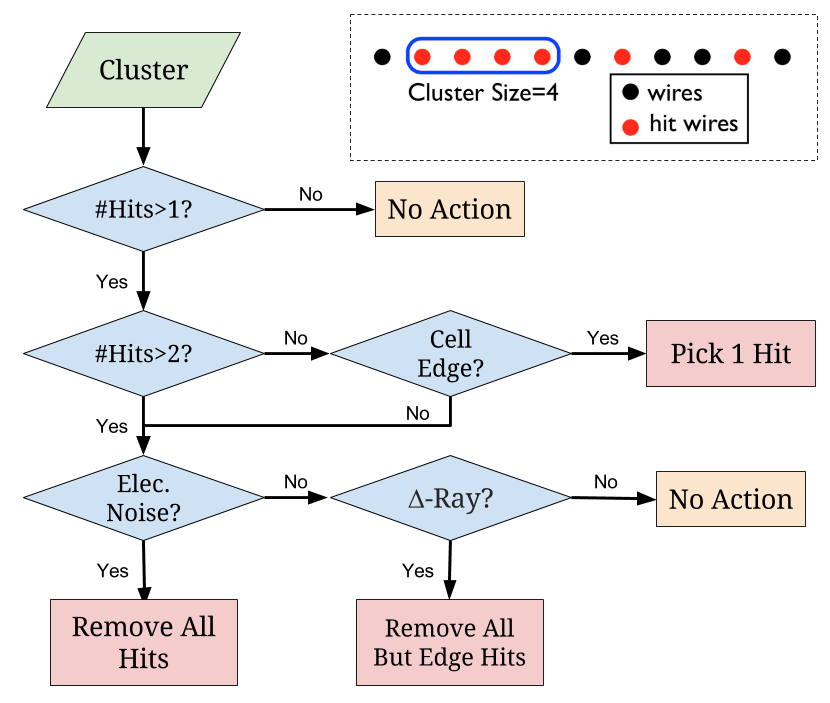
\includegraphics[height=0.25\textheight]{figures/analysis/cluster-flow.png}
	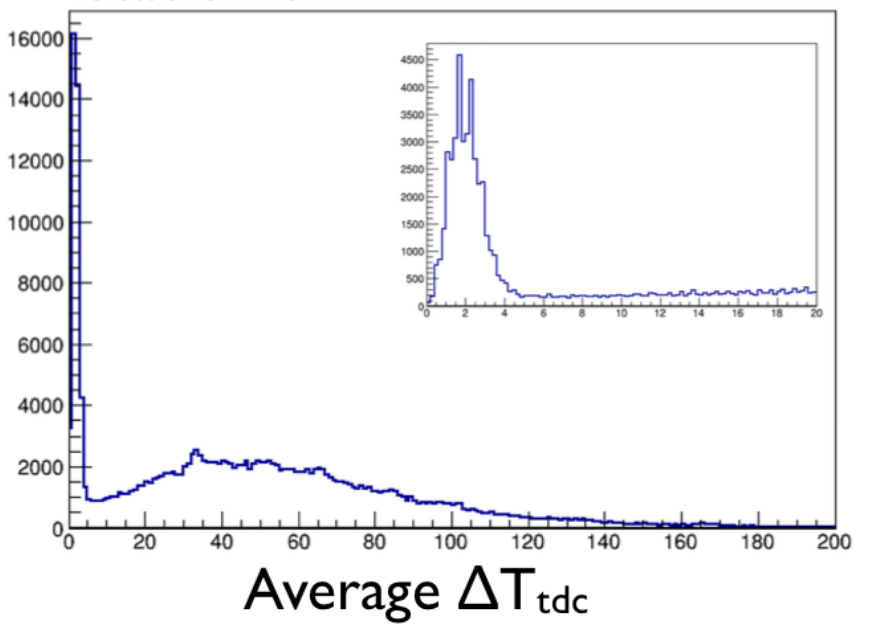
\includegraphics[height=0.25\textheight]{figures/analysis/elec-noise-cluster.png}
	\caption{(Left) A flow chart mapping out the decisions in how to treat clusters. (Right) A histogram of time differences of hits within a cluster. The peak below \unit[10]{ns} is from electronic noise, and is the deciding factor in electronic noise classification.}
	\label{fig:cluster-flow}
\end{figure}

The next type of clusters to classify is ``cell-edge'' clusters, which is defined as cases where there are two adjacent hits in a single plane where both of them have a drift distance that is greater than 90\% than the half of the cell width. In these cases, it is very likely the case that an energetic muon passed right between two sense wires, and the hit was registered by both wires. In these cases, it is advantageous to reduce the number of hits and thereby reduce the combinatoric complexity for the tracker to simply reduce the number of hits here from two down to one. The hit that is retained is the one with the smaller drift distance.

\setlength{\columnsep}{28pt}
\begin{wraptable}{r}{4cm}
	\centering
	\begin{tabular}{ll} \toprule  
		Det. Group & Hit Limit  \\ \midrule
		D1 & 250 \\  
		\rowcol D2 & 200 \\
		D3p & 150 \\
		\rowcol D3m & 120 \\
		Prop Tubes & 250 \\
		\rowcol H1T + H1B  & 10 \\
		H2T + H2B & 10 \\
		\rowcol H3T + H3B & 10 \\
		H4T + H4B & 10 \\ \bottomrule
	\end{tabular}
	\caption{The multiplicity limits imposed on detector groups by the tracking.}
	\label{tab:mult-limits}
\end{wraptable}
%------------------------------------------

The final known type of clusters that can occur are from \emph{delta-rays}, which are (relatively) low-energy knock-on electrons that scatter away along the $x-y-$plane of the detector. While these electrons are lower energy, they can still ionize the gas and incur hits in the detector. These clusters differ qualitatively from the electronic noise clusters in that, due to the speed of the traversing delta rays and the drift speed of the chamber gas, their timing difference will be $>$\unit[10]{ns} and will be missed by the electronic noise cluster removal. If a such a cluster is found, it is desired to keep the original muon hit and remove the rest of the hits incurred by the delta ray. In order to do so, the two hits on the edges of the cluster are kept while the rest are discarded.

\subsubsection{Event Removal}

\emph{After} imposing all of these data reduction methods, there is still a chance that the event's contents would make it prohibitive for tracking. The primary criteria for such classification is the \emph{multiplicity cut}. If there is an extremely large number of hits within one of the detector groups, the tracking algorithm will end up spending a very long time working through all possible combinations of hits in order to find good tracks -- too long to be considered reasonable. As such, certain multiplicity limits (shown in Table~\ref{tab:mult-limits}) are imposed on the data to abort tracking on certain events. If the occupancy of any of the detector groups exceeds the limit imposed on it, the event tracking will be aborted regardless of the occupancy of the rest of the detector groups. 

Finally, there is an additional multiplicity cut on the number of reconstructed possible \emph{trigger roads} for an event. If the in-time hodoscope hits can match five or more trigger roads of a single sign (positive or negative muon roads denoted with positive or negative roadID, respectively), then event reconstruction is aborted. In these cases, most, if not all, chamber hits in that detector half will be masked by the road masking, and it's likely the combinatorics will be too much for the tracking to reasonably handle.

\subsection{Track Finding}

Once the set of hits for a single event have been narrowed down to only the most plausibly useful hits, the next step is to begin the track finding. This consists of testing out combinations of hits between stations in order to arrive at a set of likely track candidates. The procedure for doing so can be broken down into four phases: local triplet reconstruction, St. 2-3 tracklet reconstruction, St. 1 projection of tracklets, and global track reconstruction.

The local triplet reconstruction can be thought of as the process of turning the hits of several wires in a drift chamber into a single set of $x-y$ position points within the chamber. Even further than that, a ``stub'' of a track is formed since a rudimentary slope can be estimated from the information garnered from the hits. The process begins with the combination of hits from the primed-unprimed planes. Having a pair of adjacent primed and unprimed hits allows for the elimination of the wire chamber left-right ambiguity, and better constrains the estimated position and slope. Then, all hits in the X-view is paird with all overlapping U-view hits. Those overlapping points from the X-U combinations are matched with the possible V-view hits. Each of these X-U-V combinations is then fit to an $x-y-z$-position and a slope. In forming these triplets, a single hit may be used in multiple triplets.

Once this has been done for all Station 2 and 3 hits, the set of their track stubs are matched up to form straight ``tracklets'' between the two stations. Tracklets are then kept according a certain set of criteria: if their constituent stubs sufficiently point towards each other, if the tracks vaguely point back towards the target, if the tracklet points at hodoscopes (H2, H3, and H4) that fired, and if they point to proportional tubes (3 out of 4 planes) that fired. The absorber wall between Stations 3 and 4 provide a good requirement with looking to the corresponding prop tube hits, as only muons should have made it past the iron wall and fired the prop tubes.

\begin{figure}
	\centering
	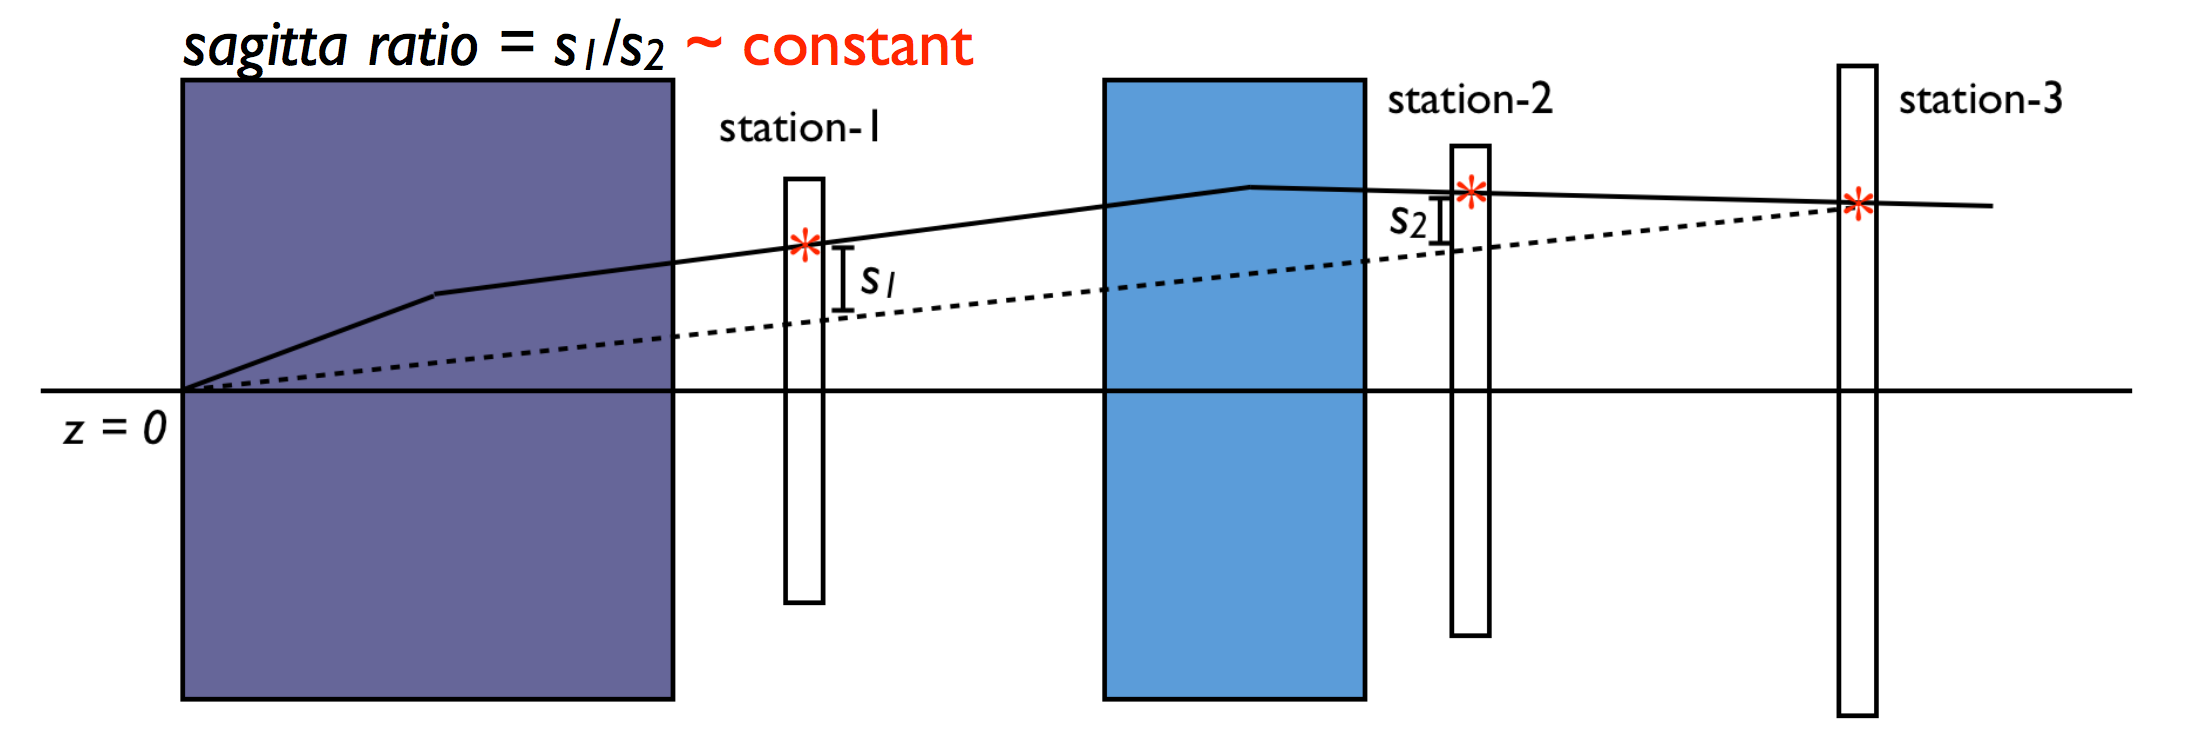
\includegraphics[height=0.17\textheight]{figures/analysis/sagitta-def.png}
	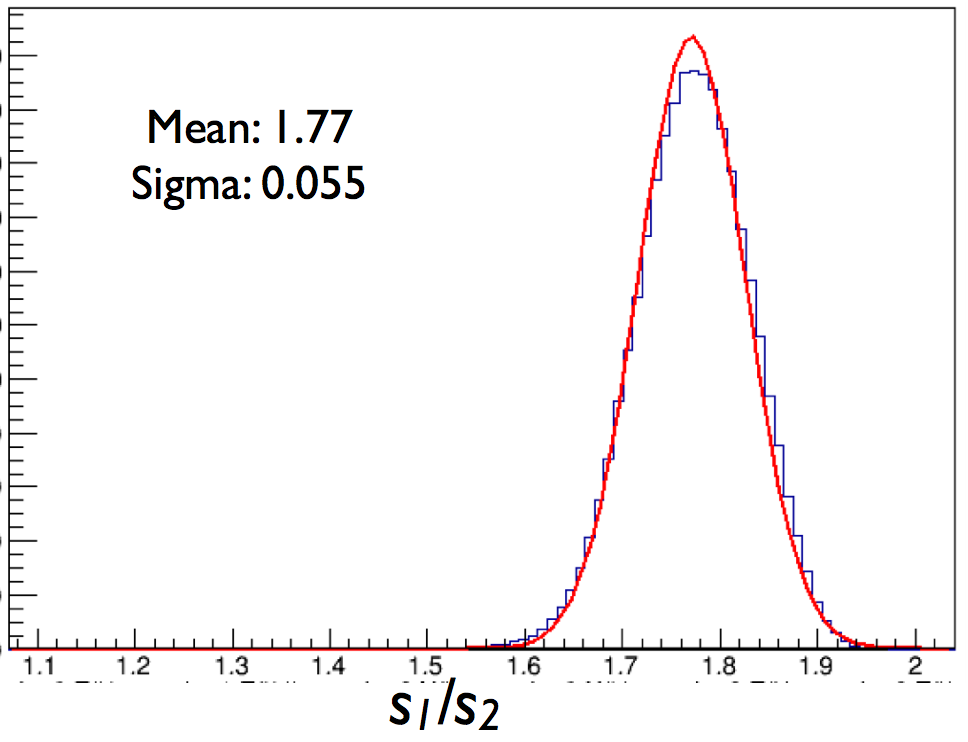
\includegraphics[height=0.17\textheight]{figures/analysis/sagitta-ratio.png}
	\caption{(Left) The definition of the sagittas $s_1$ and $s_2$, with the red asterisk denoting the actual hit positions in the stations. (Right) The ratio of the \emph{true} ratios of $s_1/s_2$ across muons of all kinda of kinematics (within acceptance) shows a single mean value with a defined variance.}
	\label{fig:sagitta-ratio}
\end{figure}

With a set of reasonable tracklets, they are each projected through KMAG and onto Station 1 to find possible matching hits there. The method by which this is done makes use of an analysis of the \emph{sagitta ratio} if known DY muon tracks.  The magnetic field of KMAG applies a $p_T-$kick of \unit[0.404]{GeV} on the muon, and the influence on its deflection is based purely on the $p_z$ of the muon at hand (assuming charge is known). As such, a large set of DY muons within the spectrometer acceptance are generated via Monte Carlo in order to measure two quantities in relation to St.3-St.1 and St.2-St.1. In Figure~\ref{fig:sagitta-ratio}, the track path of a single muon is described with the influence of the magnets being treated as a single-impulse $p_T$ kick at its center. With a line drawn between the tracklet position at Station 3 and the target ($z=x=y=0$), the quantities $s_1$ and $s_2$ are defined, which are the distances between this line and the actual hits at Station 1 and Station 2, respectively. These studies show that the ratios of these two values across various muon characteristics is distributed as a gaussian with a defined mean and variance ($\mu=1.77, \sigma=0.055$). Since this ratio and $s_2$ is known for a given tracklet, $s_1$ can be approximated and used to constrain where the hit would actually be on Station 1 within a range of $\pm$\unit[5]{cm}. With this window established, triplets are matched up at Station 1 with the tracklet in order to find candidate \emph{global tracks}.

Finally, with this set of candidate global tracks is narrowed down based on certain characteristics. This is useful as the track fitting phase which comes next is relatively intensive, so if there is any way to eliminate unlikely global tracks it should be done. The first step towards this end is the removal of hits with large \emph{residuals}, where hit residuals are defined as the difference between where the hit triplet is and where the track is projected to pass through at that $z$ position. Tracks with residuals greater than three times the resolution of the chambers are removed one at a time, with the track being refitted after each removal. Once this is done and all hits are within this acceptable residual range, then quality cuts are applied to the tracks. These cuts are (1) the hodoscope paddles along the track path must have fired, (2) the track momentum must be $5<p_{tot}<$\unit[100]{GeV}, (3) the track must have at least four hits in each station, (4) there must be at least one hit in each view (prime-unprime plane pairs) at each station, and (5) the multiple scattering in the iron absorber wall must not result in a scattering angle of more than \unit[30]{mrad}. With these quality cuts in place, the remaining tracks are passed on to the Kalman filter track fitting algorithm.

\subsection{Kalman Filter Track Fitting}

\begin{figure}
	\centering
	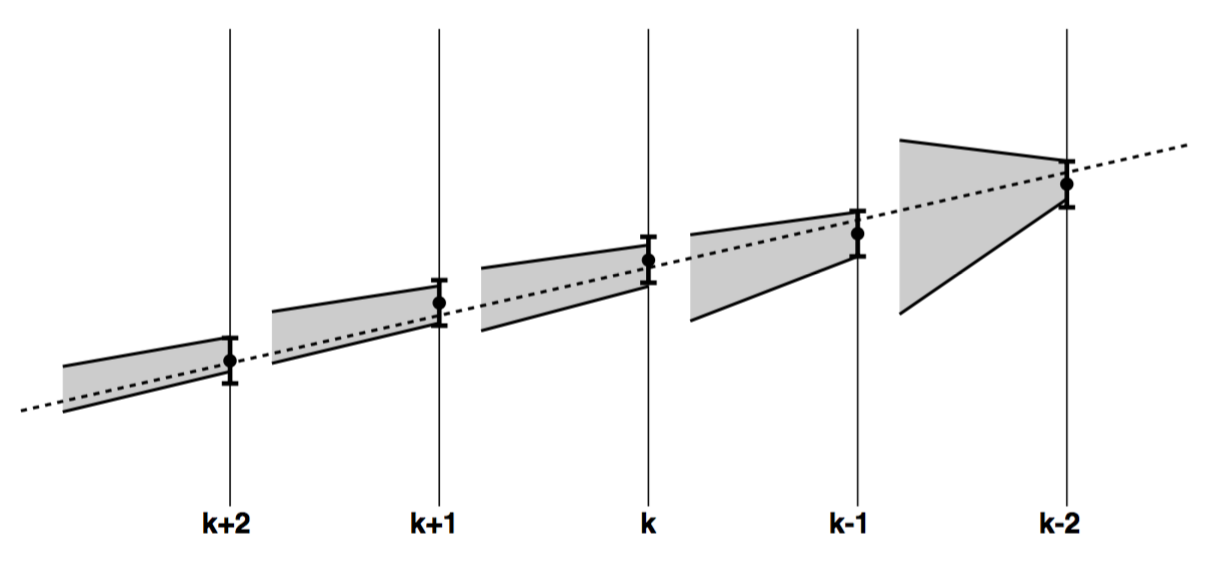
\includegraphics[height=0.3\textheight]{figures/analysis/kalman-steps.png}
	\caption{Shown is the application of the Kalman filter technique to track fitting~\cite{vanderEijk:2002sp}. The vertical lines correspond to the detector planes with indicated on it the measurement points and their errors. The cones represent the uncertainty in the reconstructed track parameters. As can be seen the knowledge of the track parameters is step wise updated with each measurement (Kalman filter technique applied from right to left).}
	\label{fig:kalman-steps}
\end{figure}

For a given track, each positional measurement throughout the spectrometer has a well-defined uncertainty to them. When these spatial information is used to reconstruct the kinematics of a muon, the sum of these \emph{fuzzy} measurements can be combined to render a better overall fit than any single measurement could make on its own. The tracking procedure has adopted an established algorithm to do just this: the \emph{Kalman Filter}\cite{kalman:1960}. The Kalman filter was developed as a signals processing algorithm to clean up a true signal out of some noisy measurements, and it has since been adapted to many different uses, including particle physics track fitting.

Before the algorithm must be applied, one must first set up a physical model that will propagate one physical state to another; in the case here, behavior of linear kineamatic motion that takes a particle from Stations 3 to 2 to 1 are defined, including the process of passing through KMAG and its fringe field. Once this is set up, the model is used to propagate the the state of the muon from one station to the other, evaluating at each step the kinematics, along with their associated uncertainties. This estimation of the measured parameters is combined with the state vector of the muon at that point to create a weighted average used to scale the measurements by their expected accuracy, which is largely dominated by the resolutions of the drift chambers. After the weighted average is calculated, the model propagates on to the next state. The algorithm repeats, ending up with a final state with a defined covariance.

Compared to the generalized Kalman Filter procedure where the propagation step is done analytically, the tracking algorithm uses Geant4 simulation to perform a dynamic state propagation from one station to another. This method is preferable for our purposes since Geant4 is well-tested and robust in its ability to handle relativistic interactions with matter and properly simulate the effects of fringe magnetic fields. Also, due to the procedure by which SeaQuest reconstructs tracks and the backwards-forwards time invariance of particle kinematics, the Kalman Filter is used to step \emph{backwards} in time. It is primarily done in this way since the downstream end of the experiment is generally ``cleaner'' than the upstream end, and the straight path between Stations 3 and 4 are generally well-defined. The Kalman algorithm is iterative, and starting out with a less uncertain starting state leads it to converge to a stable final track state faster (fewer epochs).

In the fitting of tracks, a state vector consists of the momentum and the position ($p_x, p_y, p_z, x, y, z$). The tracklets, which allow for a good starting state, are then propagated upstream towards Station 1, with the measurements being updated as more steps are taken. Figure~\ref{fig:kalman-steps} provides a depiction of stepping (from right to left) through the stations with the uncertainty in the observables updating at each step. The uncertainties of the measurements shown stem from known chamber resolutions. The propagation between Stations 2 and 1 and between Stations 1 and the target area are performed using measured magnetic field maps and Geant4 simulations of particle interactions through matter. At the projected target area, the final observables are estimated. At this point, the process is reversed, and the particle is propagated forward in time, finely adjusting the parameters to minimize the $\chi^2$ of the track. If the $\chi^2$ of the global track converges, then it is passed on to the vertex finding/fitting stage of the tracking algorithm.

\subsection{Vertex Fitting}

With the fitted global tracks, they are matched up with each other to create a two-particle vertex with all its kinematics (combined from constituent tracks) estimated, along with a goodness of fit of the tracks to the vertex itself. The vertex-finding and -fitting algorithm used in the kTracker is adapted from the approach taken by Gorbunev and Kisel at the ALICE collaboration\cite{Gorbunov:2010yda}. This approach, again, makes use of the Kalman Filter algorithm.

Before tracks can be combined to vertices, they are propagated upstream from Station 1 through FMAG via a method called a magnet `swim.' In this process, the solid iron magnet is considered as many small slices in $z$, and a commensurate amount of energy loss and $p_T-$kick is applied at each $z-$slice. Once it emerges from the upstream face of FMAG, the track is then projected as a straight line to the target region, and it is these straight segments which are used as inputs to the vertex fitting process.

In the vertex fitting, a state is defined as being the position of the (presumedly) dimuon vertex ($x_d, y_d, z_d$). This is first initialized to ($0, 0, \bar{z}$), where $\bar{z}$ is the average of all tracks' points of closest approach to the $z-$axis.
\red{talk with Evan and Jason about how track pairs are picked and vertex finding is done, then finish this subection.}

\red{Express the calculation of M, dpx, dpy, dpz, x1, x2, xF, costheta, phi, phi\_gamma from two muon momenta.}

\subsection{Monte Carlo Validation}

\begin{figure}
	\centering
	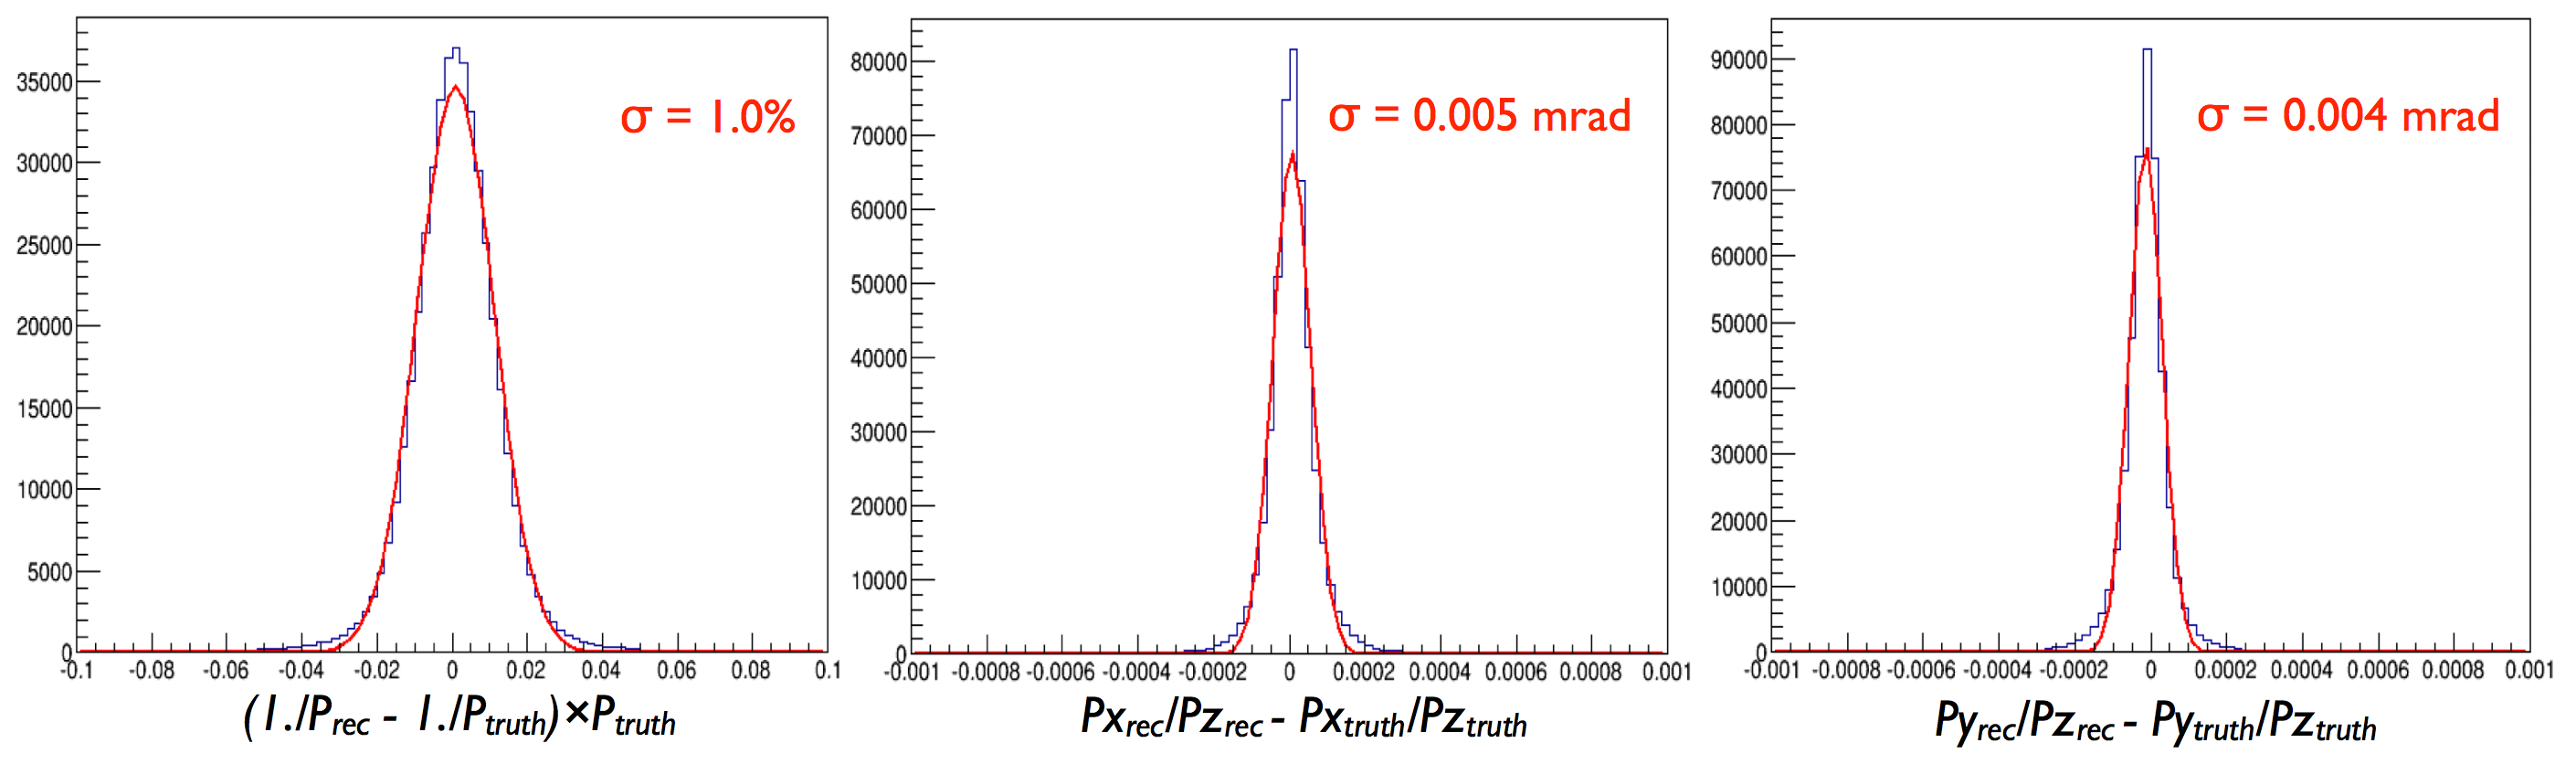
\includegraphics[width=\textwidth]{figures/analysis/track-residuals.png} \\
	\caption{The residuals of reconstructed track kinematics against MC truth values.}
	\label{fig:mc-track-validation}
	\vspace{12pt}
	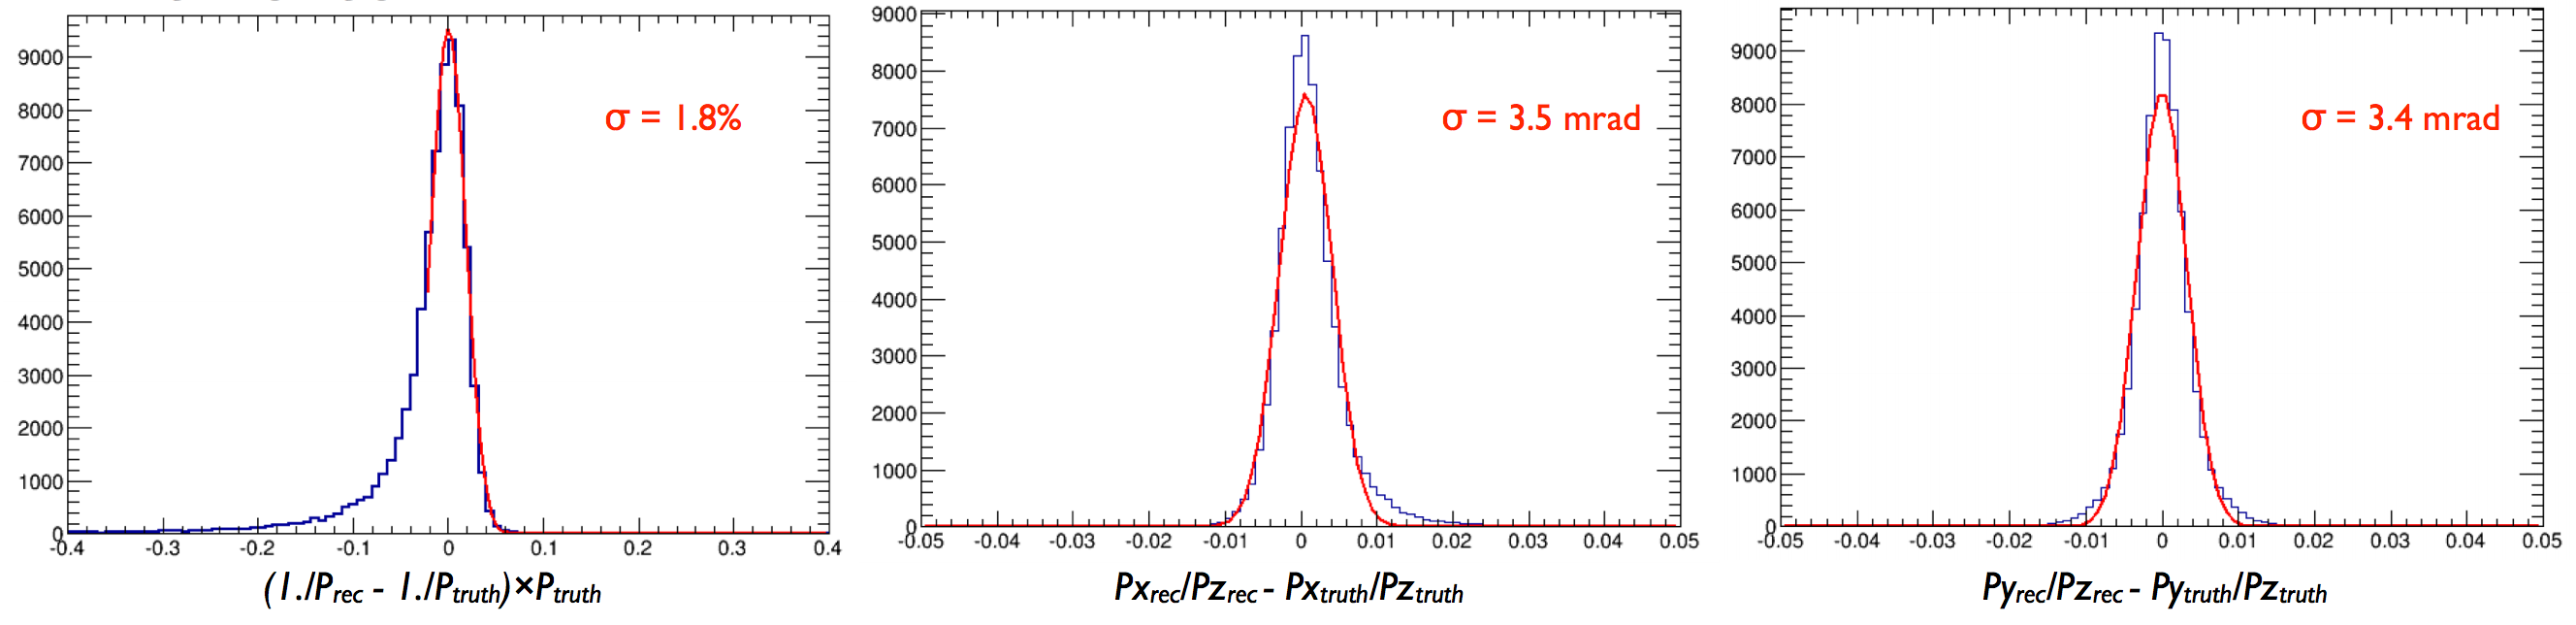
\includegraphics[width=\textwidth]{figures/analysis/dimuon-residuals.png}
	\caption{The residuals of fitted track vertex kinematics against MC truth values.}
	\label{fig:mc-vertex-validation}
\end{figure}

With the tracking algorithm established, the next logical step is to measure its accuracy and efficiency, given a sample of perfectly clean Monte Carlo generated events. These events use a geometry definition that represents the latest survey numbers describing the hall, and they also simulate the `digitization' of the hits (e.g. spatial coordinates in detectors into wire hits). Tracking is then run on these clean events to see if the developed algorithm can extract what is generated. In Figures~\ref{fig:mc-track-validation} and ~\ref{fig:mc-vertex-validation}, the residuals are shown, describing the reconstruction resolution of the track and vertex momenta. Overall, the tracking can reconstruct tracks and dimuon $p_{tot}$ within a $\sigma=1.8\%$ uncertainty. The residuals on track $p_T/p_z$ is very good ($\sigma=$\unit[0.005]{mrad}), but the effects of multiple scattering through FMAG and the vertex fitting smears out this to an residual uncertainty of $\sigma=$\unit[3.5]{mrad}.

Regarding efficiencies on clean MC, the tracking was able to find and fit two muon tracks (i.e. $\chi^2$ converged in fitting for both) at an efficiency of 92.2\% of thrown events. Once the effects of FMAG and vertex fitting is factored in, the rate at which the tracking is able to find one muon pair vertex is 69.2\%. This tracking efficiency and it's target-, kinematic- and intensity-dependence will be investigated in great depth later on in the Rate Dependence section.

\section{Analysis Cuts}\label{sec:data-cuts}

The tracking software is concerned only with reconstructing possible tracks of relativistic charged particles through the SeaQuest spectrometer. It is, however, completely agnostic as to whether or not the charged particle was a muon that originated from a Drell-Yan interaction between the beam and the target. Though the tracker is agnostic as such, it should be noted that certain measures are in place in the design of the experiment that serve to increase the chances that a reconstructed track is a true DY muon track. Such examples are the choice of trigger matrix and the construction of an absorber wall before Station 4. Despite these measures, there are many cases in which we would wish to discard some signals, events, or whole spills in order to keep the data from becoming contaminated by anything but true $p-A$ Drell-Yan target dimuons.

As such, a set of cuts must be imposed to the tracked set of dimuon yields
\begin{itemize}
	\item Drell-Yan Selection Cuts: Exclude kinematic regions where the the signal is dominated by background
	\item Target Selection Cuts: Dimuons can be created in our beam dump. These cuts seek to remove the signals that likely originate from the dump.
	\item Trigger Selection Cuts: Many triggers were used to take data, and we only wish to analyze data triggered by a certain trigger configuration.
	\item Intensity Cuts: Data taken at unusually high intensities where components of the experiment can perform abnormally should be excluded.
	\item Quality Cuts: Most cuts fall under this umbrella. These include, but are not limited to: hardware settings, DAQ quirks, dimuon/track goodness-of-fits, etc.
\end{itemize}

In this section, these cuts are discussed in the order of tiers of data taking: Run, Spill, Event, Dimuon, Track. The intent with all of these cuts is to be as conservative as possible to ensure that all possible contamination is removed from the data despite the inevitable reduction in statistics.

\subsection{Data Selection}

The first cut on analyzable data is the choice of dataset to use. This document presents and discusses the EMC ratio results for SeaQuest roadsets \#57, \#62, and \#67. Each of these roadset settings were in place for the span of months and contain varying amounts of statistics. In total, many millions of tracks and dimuons of varying quality are found through the track reconstruction and vertex fitting procedure discussed in the previous section. Several cuts regarding quality of track/dimuon fit and experimental conditions are discussed below and applied to these datasets in order to isolate signal dimuons from the \emph{target}.

The names of the SeaQuest MySQL merged productions along with their date range, magnet polarity, respective statistics, and notes regarding roadset differences are presented in Table~\ref{tab:roadset-stats}.

\begin{table}
	\centering
	\caption{The experiment-specific data sources and their details.}
	\label{tab:roadset-stats}
	\begin{tabular}{c|rrr}
		Schema & Date Range & \# Dimuons & Roadset Notes\\	
		\hline
		merged\_roadset57\_R005\_V001 & dummy & dummy & dummydummydummy \\
		merged\_roadset62\_R005\_V001 & dummy & dummy & dummydummydummy \\
		merged\_roadset67\_R005\_V001 & dummy & dummy & dummydummydummy
	\end{tabular}
\end{table}

\subsection{Run Level Cuts}

It is an outspoken goal of the SeaQuest collaboration to absolutely keep as much data as possible. This means, in general, that the largest chunk of data that we want to allow to be thrown away is on a spill-level. That withstanding, there are a certain set of factors that could lead an entire run's ($\sim$\unit[1]{hr}'s) worth of data to be excluded.

One factor is the amperage settings of the focusing and spectrometer magnets. If these are not set nominally (\unit[2000]{A} and \unit[1600]{A}, respectively), the tracking will improperly reconstruct tracks, as it depends on a specific $p_T\text{-kick}$ value from each magnet in order to discern sensible tracks from the data. For this reason, if the averaged magnet currents are below 50\% of their nominal values, the run is excluded from analysis.

Another crucial characteristic for a run is if it contains Spill values. This can be attributable to a malfunction in the Beginning of Spill / End of Spill triggers or a malfunction in the Spill Counter function. Regardless of cause, without this spill label, it becomes impossible to relate data taken to any other critical values such as target position or beam intensity.

The rest of the run-level cuts can be summarized by the umbrella term of ``DAQ issues''. If the Slow Control failed to be recorded for any reason and there are zero Beam, Target, or Environment table values in a run, it is excluded. The same goes for the BeamDAQ and Scaler readouts. Perhaps most prevalent of the DAQ issues is the case of a run that failed upon starting. These resulted in empty \unit[32]{kB} files with no usable data.

Beyond these issues, there are also ranges of runs for which there was some larger issue at hand. The best example of this is the period of data taking during Roadset 62 where the automatic target control was malfunctioning. The shift crew controlled the target position manually, but the actual target that was in the path of the beam during the spill could not be verified. As such, these runs were excluded. There is very little indication from the data itself that would incriminate itself as being untrustworthy, and so these are specifically excluded by analyzers. In practice, the runs are removed from the data set via an excluded range of spillIDs.

\subsection{Spill Level Cuts}

\begin{table}
	\centering
	\ra{1.3}
	\setlength{\tabcolsep}{2em}
	\begin{tabular}{@{}llll@{}} 
\textbf{Table} & \textbf{Value} & \textbf{Roadsets}  & \textbf{Good range} \\ \toprule
Spill & dataQuality & all & 0 \\ \cmidrule(l){2-4}
 & targetPos & all & $\in\{1,2,3,4,5,6,7\}$ \\ \midrule
Target & TARGPOS\_CONTROL & all &  = Spill table `targetPos' value \\ \midrule
Scaler & TSgo & 57, 59 & [1e3, 8e3] \\
	   & & 61 & [1e3, 1.2e4] \\
	   & & 62, 67, 70 & [1e2, 6e3] \\ \cmidrule(l){2-4}
	   & acceptedMatrix1 & 57, 59 & [1e3, 8e3] \\
	   &  & 61 & [1e3, 1.2e4] \\
	   &  & 62, 67, 70 & [1e2, 6e3] \\ \cmidrule(l){2-4}
	   & afterInhMatrix1 & 57, 59 & [1e3, 3e4] \\
	   &  & 61 & [1e3, 1e5] \\
	   &  & 62, 67, 70 & [1e2, 1e4] \\ \cmidrule(l){2-4}
	   & $\frac{\text{acceptedMatrix1}}{\text{afterInhMatrix1}}$ & 57, 59 & [0.2, 0.9] \\
       &  & 61 & [0.0, 0.9] \\
	   &  & 62, 67, 70 & [0.2, 1.05] \\ \midrule
Beam & S:G2SEM & all & [2e12, 1e13] \\ \cmidrule(l){2-4}
	 & F:NM3S (FMAG Current) & 57, 59, 62, 67, 70 & $>1000$ \\ 
 	 & & 61 & [200, 500] \\ \cmidrule(l){2-4}
 	 & F:NM4AN (KMAG Current) & all & $>1000$ \\ \midrule
BeamDAQ & QIESum & all & [4e10, 1e12] \\ \cmidrule(l){2-4}
	    & trigger\_sum\_no\_inhibit & all & [4e9, 1e11] \\ \cmidrule(l){2-4}
	    & inhibit\_block\_sum & 57, 59, 61 & [4e9, 1e11] \\
	    &  & 62, 67, 70 & [4e9, 2e11] \\ \cmidrule(l){2-4}
	    & dutyfactor53MHz & 57, 59, 61 & [15, 60] \\
	    &  & 62, 67, 70 & [10, 60] \\ \midrule
kTrack & \#Tracks/Spill & all & $>0$ \\
\bottomrule
\end{tabular}
\caption{The experiment-specific data sources and their details.}
\label{tab:spill-cuts}
\end{table}

Seeing as most of the experimental readouts pertaining to the condition of the experiment are read out only once per spill, it is a natural result that a large variety of quality cuts that are applied are evaluated at the spill level. A summar of all such cuts are summarized in Table~\ref{tab:spill-cuts}, but I will discuss a few key conditions here briefly.

One feature of a spill is the ``dutyfactor53MHz'', which is the aggregated duty factor ($\frac{\langle I\rangle^{2}}{\langle I^{2}\rangle}$) measurement over the whole spill as calculated by the Beam Intensity Monitor discussed in an earlier chapter. This an important measure that directly describes the quality of the beam provided to the experiment. A value that is too low corresponds to a spill that had the majority of its protons in just a small number of RF buckets. A duty factor value that is too high exceeds the capability of the main injector, and must therefore be erroneous. A visualization of good and bad duty factor values over a certain range of spills can be seen in Figure%~\ref{fig:dutyfactor}.

\red{add scatterplot of dutyfactor with good values in black and bad values in red to show how much they're outliers.}

The ratio of ``acceptedMatrix1'' to ``afterInhMatrix1'' is another quality factor that may not be intuitively obvious. The acceptedMatrix1 value is the number of accepted triggers recorded by the DAQ, and the the afterInhMatrix1 value is the total number of FPGA1-triggered events that were not inhibited by the BIM. Putting bounds on the ratio of these two allows the exclusion of two things: (1) spills with high DAQ dead time and (2) spills where, for whatever reason, only part of the spill was recorded. The latter of these could be the case if a spill was being partially recorded after data taking for a run had just begun\red{how??}.

\red{add line of 3 scatterplots of accepted, afterInh, and ratio with good values in black and bad values in red to show how much they're outliers.}

Other bounds such as the ``S:G2SEM'' and ``QIESum'' are measures of total delivered beam in units of protons and QIE, respectively. By putting bounds on these values, we avoid spills that are empty (no beam delivered) and spills that have far too much beam delivered. The lower bounds are non-zero due to a pedestal in each measurement.

\red{add both on same plot, but with a scale to bring them near each other. g2sem: good=blue, bad=violet, qiesum: good=orange, bad=reddish}

Other sweeping criteria for qualifying a spill as good are that spillID$\neq$0 and that there must be no duplicates of any of the values listed in Table~\ref{tab:spill-cuts}. It is necessary due to the relational nature of the data that there must be a real spillID by which one can determine all other spill-relevant values; cases where spillID=0 are cases in which no Spill Counter event was available, and these should be excluded. Regarding duplicate values, if such exist for one spillID, it is almost impossible which is the correct one, so the spill should not be considered.

Finally, certain periods of data taking are known by the collaboration to be problematic and not suitable for analysis. There exist periods of time where the trigger timing was off by a certain margin and degraded the efficacy of the trigger's ability to trigger on dimuon events. There's also a range of spills for which the magnets were flipped before a new trigger roadset could be devised for such a configuration. These are defined as a series of ``bad spill ranges'' and can be found summarized in Table~\ref{tab:spill-ranges}.

As briefly described in the chapter on database design, the addition of a ``dataQuality'' field was touched on. Here, this field is used as a bitmask in order to identify whether or not a spill passes or fails a given cut by flagging a bit as 0 (pass) or 1 (fail). This allows for analyzers to easily select only spills that pass all criteria by simply requiring \emph{dataQuality = 0}.

\begin{table}
	\centering
	\ra{1.2}
	\setlength{\tabcolsep}{2em}
	\begin{tabular}{LLl} 
		\textbf{Min SpillID} & \textbf{Max SpillID} & \textbf{Details} \\ \toprule
\rowcol 371870 & 376533 & Trigger timing shift \\
378366 & 379333 & Trigger timing shift \\
\rowcol 394287 & 409540 & Run 3 commissioning period \\
394287 & 414555 & LD2 flask filled with LH2 \\
\rowcol 416207 & 424180 & Manual target control \\
482574 & 484924 & Magnet flipped before roadset changed \\
\rowcol 526201 & 526364 & Improper QIE inhibit setting \\
581369 & 582460 & KMag off \\
\rowcol 675814 & 684041 & Drift Chamber 1 gas flow problem \\
684663 & 689443 & Incorrect D3p in-time window \\ \bottomrule
\end{tabular}
\caption{Specific spill ranges of excluded data for all roadsets.}
\label{tab:spill-ranges}
\end{table}

\subsection{Event Level Cuts}

The bare minimum requirement for the Event level data is that it must have an entry in all event-level tables: Event, kEvent (the kTracker's event meta-data), and QIE. If any of these is missing, then the event is discarded. More specific criteria can be imposed to consider an entry to be ``missing,'' such as when a row in the QIE table reports all ``-1'' values for the BIM RF readouts. In these instances, there was a malfunction in the BIM, and the ``-1'' acts as a \emph{sentinel value} to indicate that the information does not exist for that event.

In addition to missing data, certain criteria can be placed on the Event data in order to exclude poor-quality or unwanted events. The simplest cut that is imposed is the requirement that the event that was triggered must have satisfied the FPGA-1 trigger. The different trigger configurations are are designed on optimized for different purposes; the FPGA-1 trigger is designed to select high-signal, low-background Drell-Yan (opposite sign muon pair) events, and by removing other types of triggers such as the NIM-3 (random RF) and FPGA-4 (singles) that exist in the data, it is ensured that there will be no effect due to different triggering systems when performing analysis.

The cut on beam intensity is another that ensures that we exclude data that would introduce undue volatility and uncertainty into the measurements. Due to the varying beam intensity at SeaQuest, there are inefficiencies which are corrected via weighting of events (this process is described in great detail later). Cutting on very high intensities removes the region where uncertainties in the rate dependence fits can cause large uncertainties in correction weights. 

The cuts described here and more are summarized in Table~\ref{tab:all-other-cuts}.

\subsection{Dimuon Cuts}

Dimuons are selected based on many criteria: the known acceptance of the spectrometer, physical contraints, goodness of vertex fits, and more. The precise description can be summarized by the following: we are looking for two tracks of particles with opposite signs that can be \emph{well-fit} to originating from the target table. Stepping through the cuts and their justifications:

\begin{itemize}
	\item \textbf{dx, dy, dz}: These define the fitted point of origin (``dimuon (x, y, z)'') for the dimuon pair. If the vertex was outside the (dx, dy) region about the beam path, then this is probably not a real dimuon. If it it outside the desired dz range, then it probably did not come from the target.
	\item \textbf{dpx, dpy, dpz}: These define the total momentum of the dimuon (``dimuon momentum ($p_x, p_y, p_z$)). If $|p_{x/y}|>$\unit[2]{GeV}, then one or both muons would pass outside of the acceptance of the experiment. Likewise, if $|p_{z}|<$\unit[30]{GeV}, one or both of the muons would have such low momentum as to end up bent out of acceptance of the spectrometer by the magnets. Finally, since a \unit[120]{GeV} proton beam is used for SeaQuest $p_{z}>$\unit[120]{GeV} must only come from unrelated muons that are reconstructed to this high momentum value.
	\item \textbf{sgn(px1), sgn(px2)}: These are terms for the momentum of the positive and negative track, respectively. Requiring a specific sign for the $x$-momentum for each track acts as a safety check that the tracking identified the charge of the particle correctly.
	\item \textbf{sgn(roadID1), sgn(roadID2)}: This is another check that ensures that the muons came from opposite sides of the experiment (top-bottom). Such should be the case when triggered by a FPGA-1 event, but this enforces it.
	\item \textbf{trackSeparation, chisq\_dimuon}: These are measures of the goodness of fit that two tracks came together to form at a single vertex. The track separation is the distance between the points of closest approach from each track to the beam axis (z-axis). The $\chi^2_{\text{dimuon}}$ is a measure of the quality of tracks combined with how well the two tracks converge to a single point.
	\item \textbf{mass}: There is a di-lepton range of invariant masses that are book-ended by the $\Jpsi$ and the $\Upsilon$ in which Drell-Yan should be the only source. A cut on this range excludes any background that would be introduced by real $\Jpsi$s and $\Upsilon$s.
\end{itemize}

\subsection{Track Cuts}

Going even deeper to remove signal contamination, if one of the two tracks for even a \emph{good} dimuon is found to fail certain checks, the entire event is excluded from analysis. Again, stepping through each cut:
\begin{itemize}
	\item \textbf{numHits}: A track passes through 18 drift chamber planes. Even if the chambers are somewhat inefficient, it is unlikely that the number of hits corresponding to a single track would be less than 15.
	\item \textbf{roadID$\neq$0}: It is possible that a reconstructed track passes from the top half of the experiment to the bottom (and perhaps bends back up to the top). By the roadID naming convention, these are assigned a roadID of 0, and since we are looking to only analyze cases where there is one ``top'' track and one ``bottom'' track, these should be excluded. By imposing this requirement, such tracks are removed.
	\item \textbf{chisq/(numHits-5)}: Each track is described as a muon with five physical parameters ($x_1, x_2, p_T, \theta, \phi$). This expression described the $\chi^2$ per degree of freedom, and can be cut on to select only good quality tracks that fit the hit pattern well.
	\item \textbf{pz1}: This is the momentum of the track at Station 1. In studies of signal background sources, one of the primary contributors is combinatorial background, which can be analyzed by looking to like-sign triggered events and studying their kinematics. As can be seen in Figure~\ref{fig:likesign-pz-cut}, depending on the number of hits, applying a cut on pz1 can remove the strong peak of combinatoric background from unrelated muons.
	\item \textbf{chisq\_dump-chisq\_target}: These are the $\chi^2$s of a track when forced to go through the beam dump and the target, respectively. By requiring this quantity to be above a certain value means, roughly speaking, that the track is very likely to have come from the target and not the beam dump. 
\end{itemize}

\begin{figure}
	\centering
	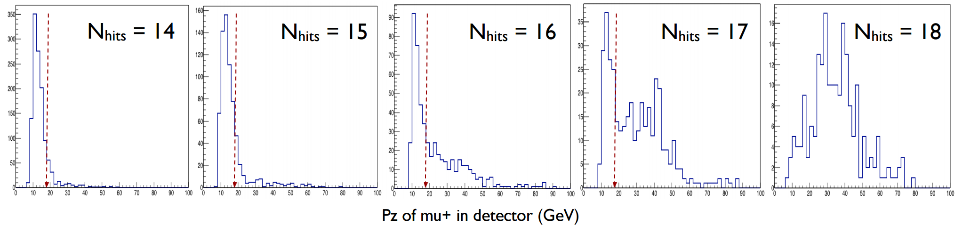
\includegraphics[width=\textwidth]{figures/analysis/likesign-pz-cut.png}
	\caption{The $p_z$ distribution of muons that form like-sign dimuon pairs, which is a source of background for DY signal events. In cases where $14\leq\text{numHits}<18$, imposing a cut on $p_z>$\unit[18]{GeV} removes a majority of this background.}
	\label{fig:likesign-pz-cut}
\end{figure}

\begin{table}
	\centering
	\ra{1.1}
	\begin{tabular}{@{}llll@{}} \midrule
		\textbf{Table} & \textbf{Value}  & \textbf{Good range} & \textbf{Type} \\ \toprule
kTrack & numHits & $>14$ & Quality \\
 & roadID & $\neq0$ & Quality \\
 & z0  & (-400, 200)  & Quality \\
 & chisq/(numHits - 5) & $<5$ & Quality \\
 & pz1 (Where numHits $\neq$ 18) & $>18$ & Quality \\
 & chisq\_dump - chisq\_target & $>10$ & Target \\ \midrule
kDimuon & dx & (-2, 2)  & Quality \\
 & dy & (-2, 2)  & Quality \\
 & dz & (-300, 200)  & Quality \\
 & dpx & (-3, 3)  & Quality \\
 & dpy & (-3, 3)  & Quality \\
 & dpz & (30, 120)  & Quality \\
 & xB & (0, 1)  & Quality \\
 & xT & (0, 1)  & Quality \\
 & xF & (-1, 1)  & Quality \\
 & trackSeparation & (-250, 250)  & Quality \\
 & chisq\_dimuon & $<15$ & Quality \\
 & px1 & $>0$ & Quality \\
 & px2 & $<0$ & Quality \\
 & dz & (-300, -60)  & Target \\
 & mass & $>4.2$ & Drell-Yan \\ \midrule
Event & MATRIX1 & 1 & Trigger \\ \midrule
kEvent & status & 0 & Quality \\ \midrule
QIE & $\forall$(RF+08, RF+07, \ldots RF-08) & $<$ Beam.Inh\_thres & Quality \\
 & $\forall$(RF$\pm XY$) & $>0$ & Quality \\
 & triggerCount & $\geq0$ & Quality \\
 & intensity\_p & $<60000$ & Quality \\
\bottomrule
\end{tabular}
\caption{A list of all quality and kinematic cuts for selecting good quality dimuons from the target.}
\label{tab:all-other-cuts}
\end{table}